\documentclass[11pt]{article}
\usepackage[a4paper,margin=2.3cm]{geometry}
\usepackage{booktabs,graphicx,longtable,caption,amsmath}
\usepackage[dvipsnames]{xcolor}
\captionsetup{font=small,labelfont=bf}
\renewcommand{\arraystretch}{1.15}
\begin{document}
\begin{center}{\Large\bfseries Rovibrational analysis: Li\_Omega}\\[2pt]
{\small Sinc-DVR (Colbert--Miller) + sixth-degree Rydberg potential}\end{center}
\noindent Reduced mass $\mu = 12522.30592\ m_e$ (6.86949 amu). Grid: 500 sinc-DVR points on the CSV range. Level count is automatic: all bound states below $D_e$.
 Input read in bohr / hartree (detected), converted to bohr / hartree.
\vspace{4pt}
\begin{table}[h]\centering\caption{Optimized sixth-degree Rydberg parameters (atomic units unless noted).}
\begin{tabular}{l r}\toprule Parameter & Value \\\midrule
$R_e$ (bohr) & 3.314473 \\
$R_e$ (\AA) & 1.753944 \\
$D_e$ (hartree) & 0.08139736 \\
$D_e$ (cm$^{-1}$) & 17864.656 \\
$D_e$ (kcal mol$^{-1}$) & 51.0776 \\
$V(R_e)$ (hartree) & -0.08385014 \\
$c_1$ & 0.64445265 \\
$c_2$ & -0.04457551 \\
$c_3$ & -0.00346911 \\
$c_4$ & 0.00837446 \\
$c_5$ & -0.00100194 \\
$c_6$ & 0.00006553 \\
fit RMS (hartree) & 8.493e-06 \\
\bottomrule\end{tabular}\end{table}
\begin{longtable}{r r r r r}
\caption{Vibrational energy levels, spectrum $E_v-E_0$ and level differences $\Delta E_v$ (cm$^{-1}$).}\\
\toprule $v$ & $E_v$ (J=0) & $E_v$ (J=1) & $E_v-E_0$ (J=0) & $\Delta E_v$ (J=0) \\\midrule\endfirsthead
\toprule $v$ & $E_v$ (J=0) & $E_v$ (J=1) & $E_v-E_0$ (J=0) & $\Delta E_v$ (J=0) \\\midrule\endhead
0 & 198.0026 & 199.5931 & 0.0000 & 392.7591 \\
1 & 590.7617 & 592.3422 & 392.7591 & 388.0596 \\
2 & 978.8212 & 980.3916 & 780.8186 & 383.3352 \\
3 & 1362.1564 & 1363.7164 & 1164.1538 & 378.5857 \\
4 & 1740.7420 & 1742.2914 & 1542.7395 & 373.8109 \\
5 & 2114.5530 & 2116.0914 & 1916.5504 & 369.0107 \\
6 & 2483.5636 & 2485.0910 & 2285.5611 & 364.1849 \\
7 & 2847.7485 & 2849.2645 & 2649.7460 & 359.3334 \\
8 & 3207.0819 & 3208.5862 & 3009.0793 & 354.4561 \\
9 & 3561.5380 & 3563.0304 & 3363.5354 & 349.5530 \\
10 & 3911.0910 & 3912.5711 & 3713.0884 & 344.6240 \\
11 & 4255.7149 & 4257.1826 & 4057.7124 & 339.6692 \\
12 & 4595.3841 & 4596.8391 & 4397.3816 & 334.6887 \\
13 & 4930.0728 & 4931.5148 & 4732.0703 & 329.6826 \\
14 & 5259.7555 & 5261.1842 & 5061.7529 & 324.6512 \\
15 & 5584.4067 & 5585.8218 & 5386.4041 & 319.5947 \\
16 & 5904.0014 & 5905.4027 & 5705.9988 & 314.5135 \\
17 & 6218.5150 & 6219.9021 & 6020.5124 & 309.4081 \\
18 & 6527.9231 & 6529.2958 & 6329.9205 & 304.2790 \\
19 & 6832.2021 & 6833.5601 & 6634.1995 & 299.1268 \\
20 & 7131.3289 & 7132.6720 & 6933.3264 & 293.9525 \\
21 & 7425.2814 & 7426.6092 & 7227.2788 & 288.7568 \\
22 & 7714.0382 & 7715.3504 & 7516.0356 & 283.5408 \\
23 & 7997.5790 & 7998.8753 & 7799.5764 & 278.3059 \\
24 & 8275.8849 & 8277.1651 & 8077.8823 & 273.0533 \\
25 & 8548.9382 & 8550.2020 & 8350.9356 & 267.7848 \\
26 & 8816.7230 & 8817.9701 & 8618.7204 & 262.5021 \\
27 & 9079.2251 & 9080.4552 & 8881.2225 & 257.2073 \\
28 & 9336.4324 & 9337.6452 & 9138.4298 & 251.9026 \\
29 & 9588.3349 & 9589.5303 & 9390.3324 & 246.5906 \\
30 & 9834.9256 & 9836.1032 & 9636.9230 & 241.2742 \\
31 & 10076.1998 & 10077.3594 & 9878.1972 & 235.9566 \\
32 & 10312.1564 & 10313.2977 & 10114.1538 & 230.6410 \\
33 & 10542.7974 & 10543.9203 & 10344.7948 & 225.3314 \\
34 & 10768.1288 & 10769.2330 & 10570.1263 & 220.0319 \\
35 & 10988.1607 & 10989.2461 & 10790.1582 & 214.7469 \\
36 & 11202.9077 & 11203.9739 & 11004.9051 & 209.4812 \\
37 & 11412.3889 & 11413.4360 & 11214.3863 & 204.2401 \\
38 & 11616.6290 & 11617.6567 & 11418.6264 & 199.0288 \\
39 & 11815.6578 & 11816.6660 & 11617.6552 & 193.8534 \\
40 & 12009.5112 & 12010.4998 & 11811.5086 & 188.7197 \\
41 & 12198.2309 & 12199.1999 & 12000.2283 & 183.6341 \\
42 & 12381.8650 & 12382.8144 & 12183.8624 & 178.6031 \\
43 & 12560.4681 & 12561.3978 & 12362.4656 & 173.6332 \\
44 & 12734.1014 & 12735.0114 & 12536.0988 & 168.7311 \\
45 & 12902.8324 & 12903.7229 & 12704.8299 & 163.9032 \\
46 & 13066.7356 & 13067.6065 & 12868.7330 & 159.1560 \\
47 & 13225.8916 & 13226.7431 & 13027.8890 & 154.4955 \\
48 & 13380.3871 & 13381.2193 & 13182.3845 & 149.9276 \\
49 & 13530.3147 & 13531.1278 & 13332.3121 & 145.4575 \\
50 & 13675.7722 & 13676.5665 & 13477.7696 & 141.0900 \\
51 & 13816.8622 & 13817.6379 & 13618.8596 & 136.8291 \\
52 & 13953.6913 & 13954.4486 & 13755.6887 & 132.6781 \\
53 & 14086.3694 & 14087.1086 & 13888.3669 & 128.6397 \\
54 & 14215.0091 & 14215.7305 & 14017.0066 & 124.7156 \\
55 & 14339.7247 & 14340.4287 & 14141.7222 & 120.9068 \\
56 & 14460.6315 & 14461.3183 & 14262.6289 & 117.2134 \\
57 & 14577.8450 & 14578.5150 & 14379.8424 & 113.6351 \\
58 & 14691.4800 & 14692.1336 & 14493.4775 & 110.1704 \\
59 & 14801.6505 & 14802.2880 & 14603.6479 & 106.8177 \\
60 & 14908.4682 & 14909.0901 & 14710.4656 & 103.5747 \\
61 & 15012.0429 & 15012.6495 & 14814.0404 & 100.4387 \\
62 & 15112.4817 & 15113.0732 & 14914.4791 & 97.4067 \\
63 & 15209.8883 & 15210.4653 & 15011.8858 & 94.4755 \\
64 & 15304.3638 & 15304.9265 & 15106.3612 & 91.6417 \\
65 & 15396.0055 & 15396.5544 & 15198.0030 & 88.9022 \\
66 & 15484.9077 & 15485.4430 & 15286.9052 & 86.2535 \\
67 & 15571.1612 & 15571.6833 & 15373.1586 & 83.6924 \\
68 & 15654.8537 & 15655.3628 & 15456.8511 & 81.2160 \\
69 & 15736.0696 & 15736.5662 & 15538.0671 & 78.8212 \\
70 & 15814.8908 & 15815.3752 & 15616.8883 & 76.5054 \\
71 & 15891.3962 & 15891.8686 & 15693.3936 & 74.2659 \\
72 & 15965.6621 & 15966.1229 & 15767.6595 & 72.1005 \\
73 & 16037.7626 & 16038.2120 & 15839.7600 & 70.0069 \\
74 & 16107.7695 & 16108.2079 & 15909.7669 & 67.9831 \\
75 & 16175.7525 & 16176.1802 & 15977.7500 & 66.0270 \\
76 & 16241.7795 & 16242.1968 & 16043.7770 & 64.1368 \\
77 & 16305.9164 & 16306.3234 & 16107.9138 & 62.3107 \\
78 & 16368.2271 & 16368.6242 & 16170.2245 & 60.5468 \\
79 & 16428.7739 & 16429.1614 & 16230.7713 & 58.8432 \\
80 & 16487.6171 & 16487.9952 & 16289.6145 & 57.1979 \\
81 & 16544.8150 & 16545.1840 & 16346.8124 & 55.6090 \\
82 & 16600.4239 & 16600.7841 & 16402.4213 & 54.0742 \\
83 & 16654.4981 & 16654.8498 & 16456.4956 & 52.5915 \\
84 & 16707.0896 & 16707.4329 & 16509.0870 & 51.1583 \\
85 & 16758.2479 & 16758.5831 & 16560.2453 & 49.7723 \\
86 & 16808.0203 & 16808.3475 & 16610.0177 & 48.4309 \\
87 & 16856.4512 & 16856.7707 & 16658.4486 & 47.1315 \\
88 & 16903.5827 & 16903.8947 & 16705.5801 & 45.8713 \\
89 & 16949.4540 & 16949.7587 & 16751.4514 & 44.6484 \\
90 & 16994.1024 & 16994.4000 & 16796.0998 & 43.4662 \\
91 & 17037.5686 & 17037.8593 & 16839.5660 & 42.3651 \\
92 & 17079.9337 & 17080.2182 & 16881.9311 & 41.5290 \\
93 & 17121.4627 & 17121.7434 & 16923.4601 & 41.4052 \\
94 & 17162.8679 & 17163.1499 & 16964.8653 & -- \\
\bottomrule\end{longtable}
\begin{table}[h]\centering\caption{Spectroscopic constants (cm$^{-1}$), from finite differences of the first vibrational levels. $\alpha_e$ and $\gamma_e$ combine the spacings of each run with the $\omega_e$, $\omega_e x_e$, $\omega_e y_e$ of the J=0 run; only the J=1 column holds constants (see note). $B_e$ comes from $B_v=(E_v(J{=}1)-E_v(J{=}0))/2$.}
\begin{tabular}{l r r}\toprule Constant & J=0 & J=1 \\\midrule
$\omega_e$ & 397.4348 & 397.4251 \\
$\omega_e x_e$ & 2.33110 & 2.33122 \\
$\omega_e y_e$ & -4.1464e-03 & -4.1470e-03 \\
\midrule
$B_e$ & \multicolumn{2}{c}{0.797689} \\
$\alpha_e$ & -5.0029e-15$^{\dagger}$ & 4.8425e-03 \\
$\gamma_e$ & -1.0985e-13$^{\dagger}$ & -5.9286e-05 \\
\bottomrule\end{tabular}
\\[2pt]{\footnotesize $^{\dagger}$Consistency residual, not a constant. At J=0 the factor $J(J+1)$ vanishes and the $+4\omega_e-23\omega_ey_e$ of the formula cancels the vibrational part exactly, leaving $\sim$0. A value far from zero would mean the constants and the levels came from different runs --- which is what the legacy code printed, its $\omega_e$ being hardcoded from an earlier run.}
\end{table}
\vspace{2pt}\noindent Rovibrational levels for arbitrary $J$ follow Dunham's expansion,
\begin{equation*}\varepsilon_{v,J}=\omega_e(v+\tfrac12)-\omega_ex_e(v+\tfrac12)^2+\omega_ey_e(v+\tfrac12)^3+\left[B_e-\alpha_e(v+\tfrac12)+\gamma_e(v+\tfrac12)^2\right]J(J+1),\end{equation*}
\noindent so the DVR is diagonalized at $J=0$ and $J=1$ only and every higher $J$ is extrapolated. Over the 95 DVR levels the expansion deviates by at most 3921.7631 cm$^{-1}$ (rms 1211.5402), the cubic in $v$ being fixed by the first four levels alone. Summation limits: $v_{max}=71$ from $\varepsilon_{v,0}<D_e$, and $v_{max}=71$ from $B_v>0$, the condition for the Euler--Maclaurin rotational integral to converge.\vspace{4pt}
\begin{longtable}{r r r r r }
\caption{Rovibrational energies $\varepsilon_{v,J}$ (cm$^{-1}$) from Dunham's expansion, up to $v_{max}=71$.}\\
\toprule $v$ & $J=0$ & $J=1$ & $J=2$ & $J=3$ \\\midrule\endfirsthead
\toprule $v$ & $J=0$ & $J=1$ & $J=2$ & $J=3$ \\\midrule\endhead
0 & 198.1341 & 199.7246 & 202.9056 & 207.6771 \\
1 & 590.8932 & 592.4738 & 595.6349 & 600.3767 \\
2 & 978.9527 & 980.5232 & 983.6640 & 988.3753 \\
3 & 1362.2879 & 1363.8479 & 1366.9680 & 1371.6481 \\
4 & 1740.8738 & 1742.4232 & 1745.5220 & 1750.1701 \\
5 & 2114.6855 & 2116.2240 & 2119.3011 & 2123.9166 \\
6 & 2483.6982 & 2485.2256 & 2488.2804 & 2492.8627 \\
7 & 2847.8869 & 2849.4030 & 2852.4351 & 2856.9834 \\
8 & 3207.2269 & 3208.7314 & 3211.7404 & 3216.2538 \\
9 & 3561.6932 & 3563.1859 & 3566.1712 & 3570.6492 \\
10 & 3911.2610 & 3912.7416 & 3915.7028 & 3920.1446 \\
11 & 4255.9053 & 4257.3736 & 4260.3103 & 4264.7152 \\
12 & 4595.6013 & 4597.0571 & 4599.9687 & 4604.3360 \\
13 & 4930.3242 & 4931.7672 & 4934.6532 & 4938.9823 \\
14 & 5260.0489 & 5261.4789 & 5264.3390 & 5268.6290 \\
15 & 5584.7508 & 5586.1675 & 5589.0011 & 5593.2514 \\
16 & 5904.4048 & 5905.8081 & 5908.6147 & 5912.8245 \\
17 & 6218.9861 & 6220.3757 & 6223.1548 & 6227.3236 \\
18 & 6528.4699 & 6529.8455 & 6532.5967 & 6536.7236 \\
19 & 6832.8312 & 6834.1926 & 6836.9154 & 6840.9997 \\
20 & 7132.0451 & 7133.3921 & 7136.0861 & 7140.1271 \\
21 & 7426.0869 & 7427.4192 & 7430.0839 & 7434.0809 \\
22 & 7714.9315 & 7716.2490 & 7718.8838 & 7722.8362 \\
23 & 7998.5542 & 7999.8565 & 8002.4611 & 8006.3680 \\
24 & 8276.9301 & 8278.2170 & 8280.7909 & 8284.6516 \\
25 & 8550.0342 & 8551.3056 & 8553.8482 & 8557.6621 \\
26 & 8817.8418 & 8819.0972 & 8821.6082 & 8825.3745 \\
27 & 9080.3279 & 9081.5672 & 9084.0460 & 9087.7641 \\
28 & 9337.4676 & 9338.6906 & 9341.1367 & 9344.8058 \\
29 & 9589.2360 & 9590.4425 & 9592.8555 & 9596.4749 \\
30 & 9835.6084 & 9836.7981 & 9839.1774 & 9842.7465 \\
31 & 10076.5598 & 10077.7324 & 10080.0777 & 10083.5956 \\
32 & 10312.0653 & 10313.2206 & 10315.5314 & 10318.9975 \\
33 & 10542.1000 & 10543.2379 & 10545.5136 & 10548.9272 \\
34 & 10766.6392 & 10767.7593 & 10769.9995 & 10773.3598 \\
35 & 10985.6578 & 10986.7599 & 10988.9642 & 10992.2706 \\
36 & 11199.1311 & 11200.2150 & 11202.3828 & 11205.6345 \\
37 & 11407.0341 & 11408.0995 & 11410.2304 & 11413.4267 \\
38 & 11609.3419 & 11610.3887 & 11612.4822 & 11615.6224 \\
39 & 11806.0298 & 11807.0576 & 11809.1132 & 11812.1966 \\
40 & 11997.0727 & 11998.0813 & 12000.0986 & 12003.1246 \\
41 & 12182.4459 & 12183.4351 & 12185.4136 & 12188.3813 \\
42 & 12362.1244 & 12363.0940 & 12365.0332 & 12367.9420 \\
43 & 12536.0834 & 12537.0331 & 12538.9325 & 12541.7817 \\
44 & 12704.2980 & 12705.2276 & 12707.0868 & 12709.8755 \\
45 & 12866.7433 & 12867.6526 & 12869.4710 & 12872.1987 \\
46 & 13023.3945 & 13024.2831 & 13026.0604 & 13028.7263 \\
47 & 13174.2266 & 13175.0944 & 13176.8300 & 13179.4334 \\
48 & 13319.2148 & 13320.0615 & 13321.7550 & 13324.2952 \\
49 & 13458.3342 & 13459.1596 & 13460.8105 & 13463.2868 \\
50 & 13591.5599 & 13592.3638 & 13593.9716 & 13596.3833 \\
51 & 13718.8671 & 13719.6492 & 13721.2134 & 13723.5598 \\
52 & 13840.2308 & 13840.9909 & 13842.5111 & 13844.7914 \\
53 & 13955.6263 & 13956.3641 & 13957.8398 & 13960.0533 \\
54 & 14065.0285 & 14065.7439 & 14067.1746 & 14069.3206 \\
55 & 14168.4127 & 14169.1053 & 14170.4906 & 14172.5684 \\
56 & 14265.7539 & 14266.4236 & 14267.7629 & 14269.7719 \\
57 & 14357.0274 & 14357.6738 & 14358.9667 & 14360.9061 \\
58 & 14442.2081 & 14442.8311 & 14444.0771 & 14445.9462 \\
59 & 14521.2712 & 14521.8706 & 14523.0693 & 14524.8673 \\
60 & 14594.1919 & 14594.7674 & 14595.9182 & 14597.6445 \\
61 & 14660.9453 & 14661.4966 & 14662.5991 & 14664.2529 \\
62 & 14721.5064 & 14722.0333 & 14723.0871 & 14724.6677 \\
63 & 14775.8505 & 14776.3527 & 14777.3573 & 14778.8641 \\
64 & 14823.9526 & 14824.4300 & 14825.3848 & 14826.8170 \\
65 & 14865.7878 & 14866.2401 & 14867.1447 & 14868.5016 \\
66 & 14901.3313 & 14901.7583 & 14902.6122 & 14903.8931 \\
67 & 14930.5582 & 14930.9596 & 14931.7624 & 14932.9666 \\
68 & 14953.4437 & 14953.8193 & 14954.5704 & 14955.6972 \\
69 & 14969.9628 & 14970.3123 & 14971.0114 & 14972.0599 \\
70 & 14980.0906 & 14980.4138 & 14981.0603 & 14982.0301 \\
71 & 14983.8023 & 14984.0991 & 14984.6925 & 14985.5827 \\
\bottomrule\end{longtable}
\begin{figure}[h]\centering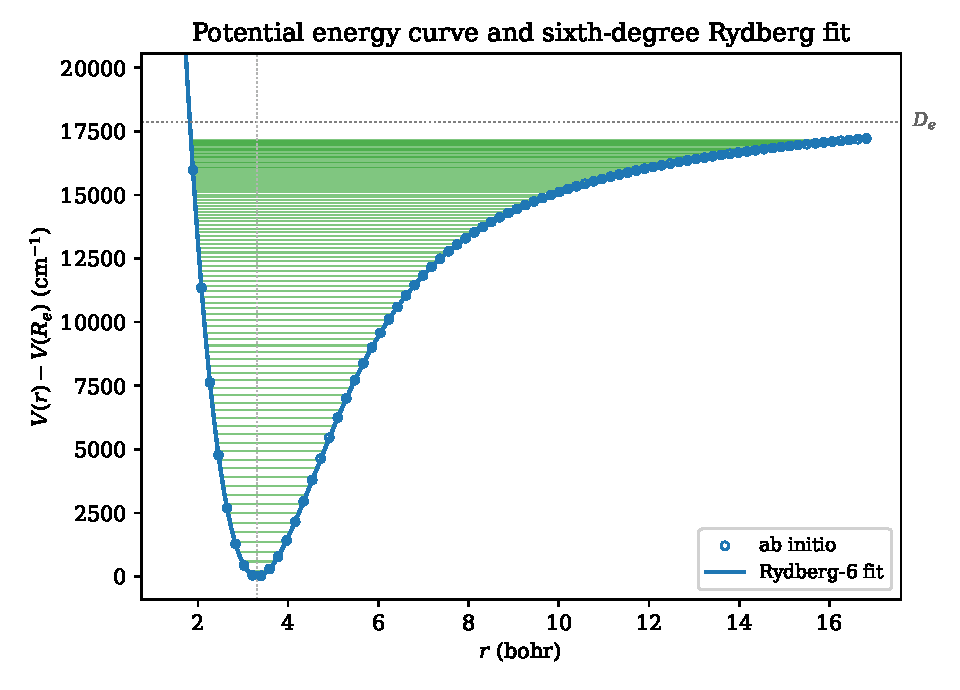
\includegraphics[width=0.82\textwidth]{Li_Omega_assets/pec.pdf}
\caption{Potential energy curve: ab initio points, sixth-degree Rydberg fit, and the J=0 vibrational levels (green).}\end{figure}
\begin{figure}[h]\centering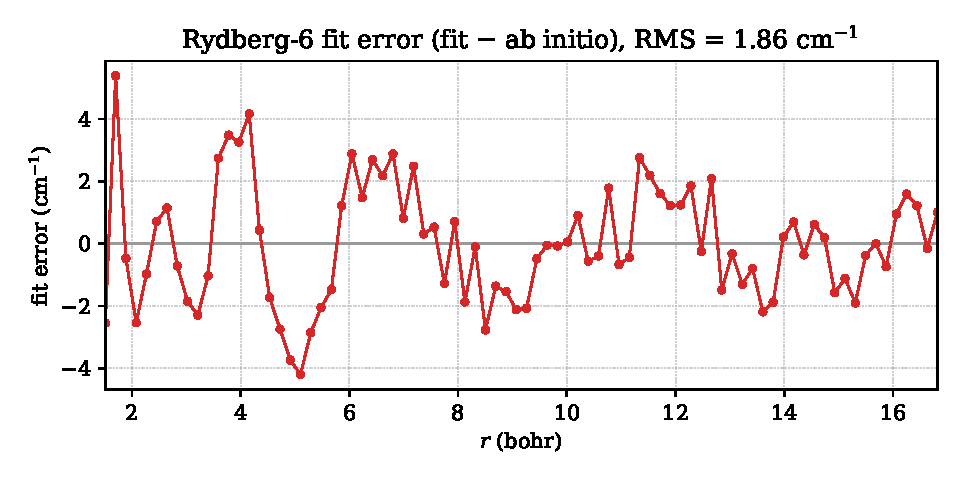
\includegraphics[width=0.82\textwidth]{Li_Omega_assets/fiterror.pdf}
\caption{Residual of the sixth-degree Rydberg fit, fit $-$ ab initio, over the whole grid.}\end{figure}
\begin{figure}[h]\centering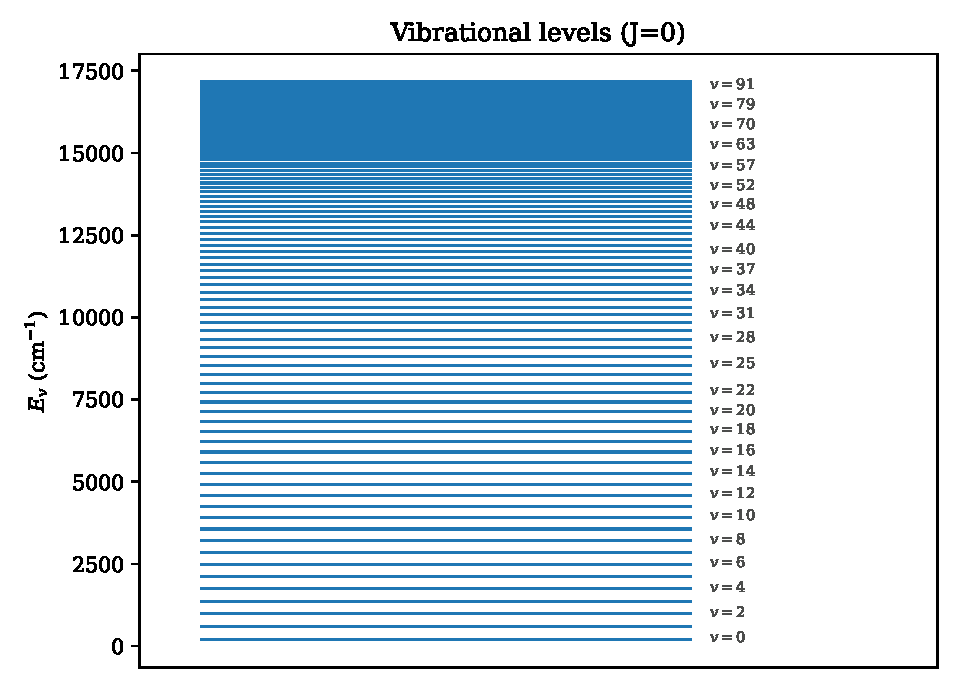
\includegraphics[width=0.82\textwidth]{Li_Omega_assets/ladder.pdf}
\caption{Vibrational energy-level ladder of the J=0 run: every bound state below $D_e$, labelled where the spacing allows.}\end{figure}
\begin{figure}[h]\centering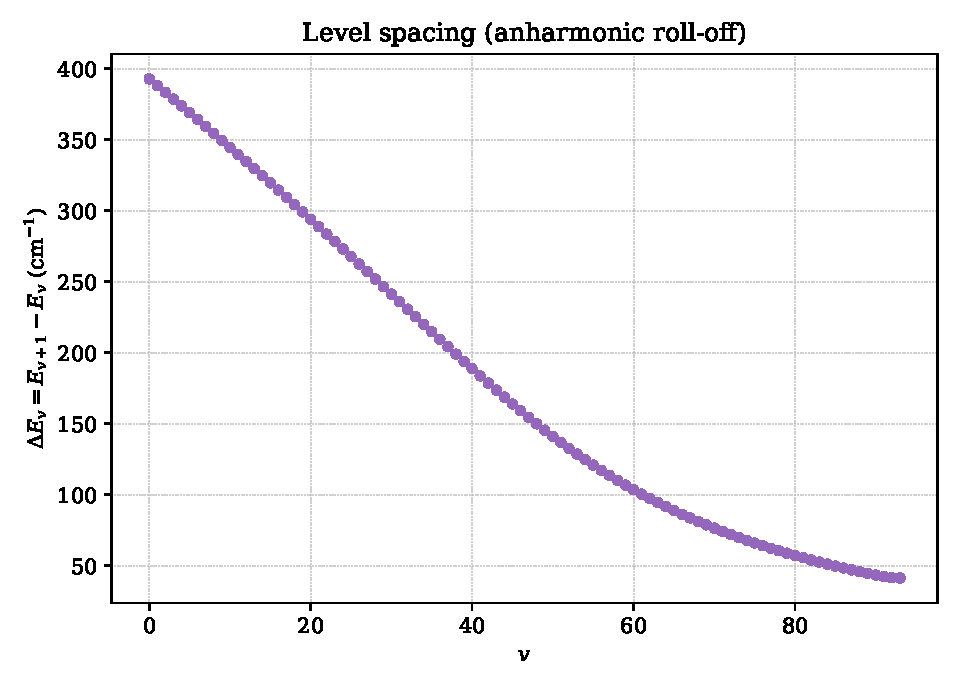
\includegraphics[width=0.82\textwidth]{Li_Omega_assets/spacing.pdf}
\caption{Anharmonic decrease of the level spacing $\Delta E_v=E_{v+1}-E_v$ with $v$, up to dissociation.}\end{figure}
\end{document}